% arara: xelatex: { options: ["--synctex=1", "-interaction=nonstopmode", "-output-directory=../build"] }
% arara: biber: { options: ["--output-directory=../build", "../build/report"] }
% arara: xelatex: { options: ['-synctex=1', '-interaction=nonstopmode', '-output-directory=../build'] }
% arara: xelatex: { options: ['-synctex=1', '-interaction=nonstopmode', '-output-directory=../build'] }
% arara: move: { files: ["../build/report.pdf"], target: "../pdf/" }

\documentclass[aspectratio=169,10pt]{beamer}
\usepackage{graphicx}
\usepackage{amssymb,amsfonts,amsmath}
\usepackage{array}
\usepackage{xeCJK}
\usepackage{tcolorbox}
\usepackage{tikz}
\usetikzlibrary{positioning}
\usepackage{pifont}
\setCJKmainfont{STSong}
\setCJKsansfont{STHeiti}
\setCJKmonofont{STFangsong}
\usefonttheme[onlymath]{serif}

% 自定义颜色
\definecolor{highlightyellow}{RGB}{255, 242, 0}
\definecolor{dotred}{RGB}{200, 30, 30}
\definecolor{dotyellow}{RGB}{255, 200, 0}
\definecolor{darkgreen}{RGB}{0, 128, 0}

% biblatex with biber
\usepackage[backend=biber,style=numeric,sorting=none,firstinits=true]{biblatex}
\addbibresource{ref.bib}
\usepackage{hyperref}

% 自定义参考文献样式
\DeclareNameAlias{author}{first-last}
\DeclareBibliographyDriver{article}{%
  \printnames{author}%
  \setunit{\addspace}%
  \printfield{title}%
  \newunit
  \printfield{journaltitle}%
  \setunit{\addspace}%
  \printfield{year}%
}

% Beamer 脚注引用设置
\setbeamertemplate{footnote}{%
  \parindent 0em\noindent%
  \raggedright
  \usebeamercolor{footnote}\hbox to 0.8em{\hfil\insertfootnotemark}\insertfootnotetext\par%
}
\setbeamerfont{footnote}{size=\tiny}
\renewcommand{\footnotesize}{\tiny}

% 定义简短脚注引用命令
\DeclareCiteCommand{\footcitetext}[\mkbibfootnotetext]
  {\usebibmacro{prenote}}
  {\usebibmacro{citeindex}%
   \printnames[family-given]{labelname}%
   \setunit{\addcomma\space}%
   \printfield[citetitle]{labeltitle}%
   \setunit{\addcomma\space}%
   \printfield{year}}
  {\multicitedelim}
  {\usebibmacro{postnote}}

% 重定义 \cite 为同时显示编号和脚注
\let\oldcite\cite
\renewcommand{\cite}[1]{\oldcite{#1}\footcitetext{#1}}

\title{Context Graph 与 Agent Memory\\{\large 面向 Coding Agent 的研究方向探索}}
\author{WU Zihan}
\date{\today}

\begin{document}
\maketitle

\begin{frame}
  \frametitle{报告结构}
  \tableofcontents
\end{frame}

%==============================================================================
\section{问题背景}
%==============================================================================

\begin{frame}
  \frametitle{技术演进：从 LLM 到 Context Graph}

  \begin{center}
  \begin{tikzpicture}[node distance=0.5cm, every node/.style={align=center}]
    % 顶会配色：蓝色渐变 + 强调色
    \definecolor{stage1}{RGB}{227,242,253}  % 浅蓝
    \definecolor{stage2}{RGB}{187,222,251}  % 淡蓝
    \definecolor{stage3}{RGB}{144,202,249}  % 中蓝
    \definecolor{stage4}{RGB}{66,165,245}   % 深蓝（强调）
    \definecolor{accenttext}{RGB}{21,101,192} % 深蓝文字
    \definecolor{graytext}{RGB}{117,117,117}  % 灰色说明

    % 节点样式
    \tikzstyle{level} = [rectangle, rounded corners=3pt, minimum width=2.6cm, minimum height=1.8cm, draw=none, font=\small]
    \tikzstyle{issue} = [font=\scriptsize, text=graytext, text width=2.4cm, align=center]
    \tikzstyle{good} = [font=\scriptsize\bfseries, text=accenttext, text width=2.4cm, align=center]

    % LLM
    \node[level, fill=stage1] (llm) at (0, 0) {\textbf{LLM}\\{\scriptsize 理解语言、生成代码}};
    \node[issue, below=0.15cm of llm] {无法与外界交互\\无记忆};

    % Agent
    \node[level, fill=stage2, right=1.2cm of llm] (agent) {\textbf{Agent}\\{\scriptsize LLM + Tools}};
    \node[issue, below=0.15cm of agent] {没有记忆\\重复犯错};

    % Agent + Memory
    \node[level, fill=stage3, right=1.2cm of agent] (memory) {\textbf{Agent + Memory}\\{\scriptsize 存储历史经验}};
    \node[issue, below=0.15cm of memory] {扁平存储\\检索不精准};

    % Agent + Context Graph
    \node[level, fill=stage4, right=1.2cm of memory] (cg) {\color{white}\textbf{Agent + CG}\\{\scriptsize 结构化、可推理}};
    \node[good, below=0.15cm of cg] {研究方向};

    % 箭头
    \draw[->, thick, accenttext] (llm) -- node[above, font=\scriptsize, text=graytext] {+工具} (agent);
    \draw[->, thick, accenttext] (agent) -- node[above, font=\scriptsize, text=graytext] {+记忆} (memory);
    \draw[->, thick, accenttext] (memory) -- node[above, font=\scriptsize, text=graytext] {+图结构} (cg);
  \end{tikzpicture}
  \end{center}

  \vspace{0.3cm}

  \begin{block}{演进逻辑}
    \small
    \textbf{LLM}：强大但封闭 $\rightarrow$
    \textbf{Agent}：能行动但健忘 $\rightarrow$
    \textbf{+Memory}：能记忆但扁平 $\rightarrow$
    \textbf{+Context Graph}：结构化、可推理、可解释
  \end{block}
\end{frame}

\begin{frame}
  \frametitle{Agent 的四大问题}

  \begin{columns}[T]
    \begin{column}{0.48\textwidth}
      \begin{block}{1. 重复犯错}
        同样的错误，换个任务又犯一遍\\
        \textcolor{gray}{\small 例：每次都忘记先安装依赖}
      \end{block}

      \begin{block}{2. 不会积累经验}
        每次任务都从零开始\\
        \textcolor{gray}{\small 例：解决过的 Bug 类型不会复用}
      \end{block}
    \end{column}

    \begin{column}{0.48\textwidth}
      \begin{block}{3. 上下文爆炸}
        执行步骤多了，历史记录太长\\
        \textcolor{gray}{\small 例：超出 token 限制，性能下降}
      \end{block}

      \begin{block}{4. 无法跨任务学习}
        任务 A 学到的经验，任务 B 用不上\\
        \textcolor{gray}{\small 例：auth 模块的经验无法迁移到 payment}
      \end{block}
    \end{column}
  \end{columns}

  \vspace{0.4cm}

  \begin{alertblock}{核心需求}
    需要一种\textbf{结构化的记忆系统}，能够组织、关联、检索 Agent 的历史经验
  \end{alertblock}
\end{frame}

\begin{frame}
  \frametitle{现有方法的不足}

  \begin{columns}[T]
    \begin{column}{0.48\textwidth}
      \begin{block}{传统 RAG}
        \begin{itemize}
          \item 基于向量相似度检索
          \item \textcolor{darkgreen}{优点}：语义匹配能力强
          \item \textcolor{red}{问题}：
          \begin{itemize}
            \item 丢失实体间的逻辑关联
            \item 无法回答全局性问题
            \item 多跳推理能力弱
          \end{itemize}
        \end{itemize}
      \end{block}
    \end{column}

    \begin{column}{0.48\textwidth}
      \begin{block}{传统知识图谱}
        \begin{itemize}
          \item 结构化三元组 \texttt{(S, P, O)}
          \item \textcolor{darkgreen}{优点}：关系明确、可推理
          \item \textcolor{red}{问题}：
          \begin{itemize}
            \item 缺乏时间、来源等上下文
            \item 结构固定，难以适应新场景
            \item 难以处理非结构化信息
          \end{itemize}
        \end{itemize}
      \end{block}
    \end{column}
  \end{columns}

  \vspace{0.5cm}

  \begin{block}{需要什么？}
    结合两者优势：\textbf{图结构的关系表达} + \textbf{上下文信息的丰富性} + \textbf{动态适应能力}
  \end{block}
\end{frame}

\begin{frame}
  \frametitle{为什么用图？—— 五大优势}

  \small
  \renewcommand{\arraystretch}{1.4}
  \centering
  \begin{tabular}{>{\centering}p{1.8cm}|>{\centering}p{3.8cm}|>{\centering\arraybackslash}p{5.8cm}}
    \textbf{能力} & \textbf{问题示例} & \textbf{RAG vs Graph} \\
    \hline
    \textbf{关系建模} & Action A 之后应该做什么？ &
    RAG: 找相似文档 $\rightarrow$ 可能不相关\newline Graph: 出边直接指向下一步 $\rightarrow$ 精确 \\
    \hline
    \textbf{路径推理} & 如何从当前状态到达成功？ &
    RAG: 无"路径"概念\newline Graph: 搜索最短/最优路径 \\
    \hline
    \textbf{失败诊断} & 为什么这次失败了？ &
    RAG: 找类似案例，但不知差异\newline Graph: 比较成功/失败路径，找分叉点 \\
    \hline
    \textbf{动态更新} & 新经验如何融入？ &
    Fine-tuning: 需重训，可能遗忘\newline Graph: 增量更新节点/边 \\
    \hline
    \textbf{可解释性} & Agent 为什么这样决定？ &
    Neural: 黑盒，无法解释\newline Graph: "因为 A$\rightarrow$B 成功率 95\%" \\
  \end{tabular}
\end{frame}

%==============================================================================
\section{Context Graph 概念框架}
%==============================================================================

\begin{frame}
  \frametitle{Context Graph：定义与定位}

  \begin{block}{核心定义 \cite{foundationcapital2024context}}
    Context Graph 是由\textbf{决策痕迹}（decision traces）编织成的活体记录结构，
    将实体、时间、先例连接成可查询的网络
  \end{block}

  \vspace{0.3cm}

  \begin{block}{与传统 KG 的区别}
    \small
    \begin{tabular}{p{2.2cm}|p{4cm}|p{4.5cm}}
      \textbf{维度} & \textbf{传统 KG} & \textbf{Context Graph} \\
      \hline
      设计目标 & 人类专家查询 & AI 模型消费 \\
      核心要素 & 实体 + 关系 & 实体 + 关系 + \textbf{决策事件} \\
      时间处理 & 无或单时态 & 双时态（有效时间+事务时间） \\
      溯源机制 & 可选 & \textbf{核心组件} \\
      更新方式 & 批量导入 & 实时/增量更新 \\
    \end{tabular}
  \end{block}

  \begin{block}{技术定位}
    \small
    \textbf{学术视角}：GraphRAG 算法创新 \quad
    \textbf{产业视角}：决策痕迹捕获 \quad
    \textbf{Agent 视角}：结构化经验记忆
  \end{block}
\end{frame}

\begin{frame}
  \frametitle{GraphRAG vs Context Graph}

  \begin{alertblock}{核心论点}
    \textbf{GraphRAG 是检索技术，Context Graph 是架构愿景}。两者共享"图"结构，但解决不同层次的问题
  \end{alertblock}

  \vspace{0.1cm}

  \footnotesize
  \renewcommand{\arraystretch}{1.3}
  \centering
  \begin{tabular}{>{\centering}p{2cm}|>{\centering}p{4.3cm}|>{\centering\arraybackslash}p{4.8cm}}
    \textbf{维度} & \textbf{GraphRAG} & \textbf{Context Graph} \\
    \hline
    定位 & 检索技术 & 架构愿景 \\
    \hline
    目标 & 改进 LLM 检索质量 & 捕获决策上下文 \\
    \hline
    数据源 & 静态文档语料库 & 多系统实时状态 \\
    \hline
    时态处理 & 静态快照 & 双时态（有效时间+事务时间） \\
    \hline
    输出 & 相关文档片段 & 决策依据链 \\
    \hline
    成熟度 & \textcolor{darkgreen}{2024-2025 学术验证充分} & \textcolor{red}{需要架构层面重新设计} \\
  \end{tabular}

  \vspace{0.2cm}

  \normalsize
  \begin{block}{关系类比}
    GraphRAG 之于 Context Graph $\approx$ TCP/IP 之于互联网：\textbf{关键技术组件}，完整实现需要更多系统工程
  \end{block}
\end{frame}

\begin{frame}
  \frametitle{Context Graph 示例}

  \begin{figure}
    \centering
    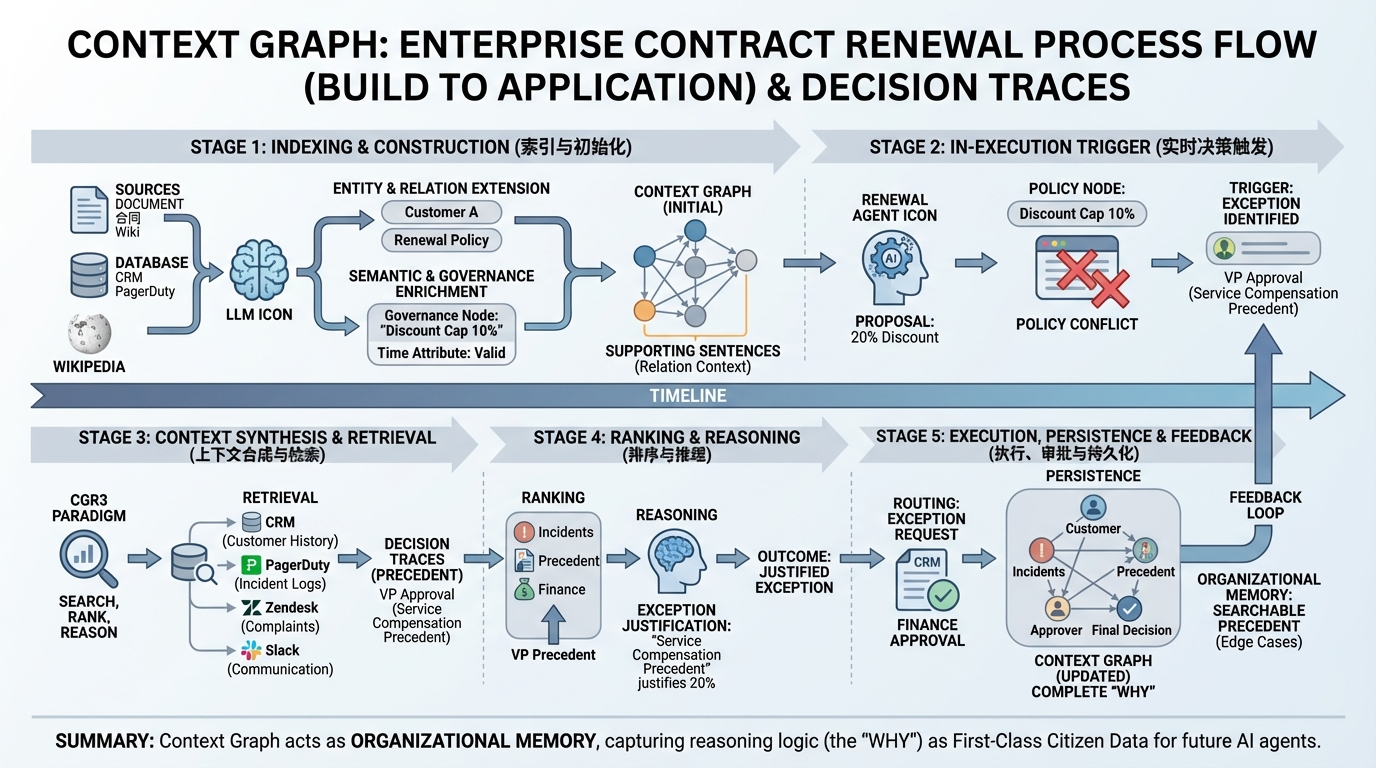
\includegraphics[width=0.85\textwidth,height=0.72\textheight,keepaspectratio]{../images/context_graph_example.jpg}
    \caption{Context Graph 如何组织决策过程与实体关系}
  \end{figure}

\end{frame}

\begin{frame}
  \frametitle{Context Graph 设计：节点与边}

  \begin{columns}[T]
    \begin{column}{0.48\textwidth}
      \begin{block}{节点类型}
        \footnotesize
        \textbf{类型 1: Action Node（动作节点）}
        \begin{itemize}
          \item \texttt{action\_type}: read\_file | write\_file | run\_test
          \item \texttt{parameters}: \{file: "auth.py", ...\}
          \item \texttt{result}: success | failure | partial
          \item \texttt{cost}: token 消耗
        \end{itemize}

        \vspace{0.2cm}

        \textbf{类型 2: State Node（状态节点）}
        \begin{itemize}
          \item \texttt{description}: "发现 bug 在 line 42"
          \item \texttt{context}: 相关文件、变量
          \item \texttt{is\_terminal}: 是否终止状态
        \end{itemize}

        \vspace{0.2cm}

        \textbf{类型 3: Insight Node（洞察节点）}
        \begin{itemize}
          \item \texttt{insight}: "Django migration 问题需先检查 models"
          \item \texttt{confidence}: 0.85
          \item \texttt{source\_tasks}: [task\_1, task\_2, ...]
        \end{itemize}
      \end{block}
    \end{column}

    \begin{column}{0.48\textwidth}
      \begin{block}{边类型}
        \footnotesize
        \textbf{类型 1: NEXT（时序/因果）}
        \begin{itemize}
          \item Action\_A $\xrightarrow{\text{NEXT}}$ Action\_B
          \item 属性: success\_rate, avg\_reward, count
        \end{itemize}

        \vspace{0.2cm}

        \textbf{类型 2: CAUSES（因果）}
        \begin{itemize}
          \item Action\_X $\xrightarrow{\text{CAUSES}}$ Failure\_Y
          \item "修改了 config 导致测试失败"
        \end{itemize}

        \vspace{0.2cm}

        \textbf{类型 3: SIMILAR\_TO（相似）}
        \begin{itemize}
          \item Task\_1 $\xrightarrow{\text{SIMILAR\_TO}}$ Task\_2
          \item 用于检索相似任务的经验
        \end{itemize}

        \vspace{0.2cm}

        \textbf{类型 4: ABSTRACTS（抽象）}
        \begin{itemize}
          \item [Action\_1, Action\_2, ...] $\rightarrow$ Insight
          \item 多个具体经验抽象成通用规则
        \end{itemize}
      \end{block}
    \end{column}
  \end{columns}
\end{frame}

%==============================================================================
\section{相关技术}
%==============================================================================

\begin{frame}
  \frametitle{技术路线图}

  \begin{figure}
    \centering
    \begin{tikzpicture}[scale=0.85]
      % 顶会配色：蓝色渐变
      \definecolor{rootcolor}{RGB}{66,165,245}    % 深蓝（强调）
      \definecolor{branch1}{RGB}{144,202,249}     % 中蓝
      \definecolor{branch2}{RGB}{129,199,132}     % 绿色
      \definecolor{leaf1}{RGB}{187,222,251}       % 淡蓝
      \definecolor{leaf2}{RGB}{200,230,201}       % 淡绿
      \definecolor{linecolor}{RGB}{21,101,192}    % 深蓝线条

      % 定义样式 - 缩小叶节点宽度避免重叠
      \tikzstyle{box} = [rectangle, rounded corners=3pt, minimum width=2.2cm, minimum height=0.8cm, text centered, draw=none]
      \tikzstyle{leafbox} = [rectangle, rounded corners=3pt, minimum width=1.9cm, minimum height=0.7cm, text centered, draw=none, font=\small]

      % 第一层：问题
      \node[box, fill=rootcolor, text=white, font=\bfseries] (problem) at (0, 3) {Agent 需要记忆};

      % 第二层：两条路线
      \node[box, fill=branch1] (graphrag) at (-4, 1.5) {图增强检索};
      \node[box, fill=branch2] (memory) at (4, 1.5) {Agent Memory};

      % 第三层：具体方法 - 增大间距
      \node[leafbox, fill=leaf1] (grag1) at (-6.2, 0) {GraphRAG};
      \node[leafbox, fill=leaf1] (grag2) at (-4, 0) {CGR³};
      \node[leafbox, fill=leaf1] (grag3) at (-1.8, 0) {GoR};

      \node[leafbox, fill=leaf2] (mem1) at (1.8, 0) {ExpeL};
      \node[leafbox, fill=leaf2] (mem2) at (4, 0) {A-Mem};
      \node[leafbox, fill=leaf2] (mem3) at (6.5, 0) {\scriptsize 可训练图记忆};

      % 连线
      \draw[->, thick, linecolor] (problem) -- (-2, 1.5) -- (graphrag);
      \draw[->, thick, linecolor] (problem) -- (2, 1.5) -- (memory);
      \draw[->, linecolor] (graphrag) -- (grag1);
      \draw[->, linecolor] (graphrag) -- (grag2);
      \draw[->, linecolor] (graphrag) -- (grag3);
      \draw[->, linecolor] (memory) -- (mem1);
      \draw[->, linecolor] (memory) -- (mem2);
      \draw[->, linecolor] (memory) -- (mem3);
    \end{tikzpicture}
  \end{figure}

  \vspace{0.3cm}

  \begin{block}{两条技术路线}
    \begin{itemize}
      \item \textbf{图增强检索}：用图结构改进 RAG 的检索质量（偏向信息检索）
      \item \textbf{Agent Memory}：为 Agent 构建可学习的经验系统（偏向智能体）
    \end{itemize}
  \end{block}
\end{frame}

\begin{frame}
  \frametitle{图增强检索：Microsoft GraphRAG \cite{microsoft2024graphrag}}

  \begin{columns}[T]
    \begin{column}{0.42\textwidth}
      \small
      \begin{block}{核心问题}
        传统 RAG 无法回答全局性问题：\\
        "这个语料库在讨论什么主题？"
      \end{block}

      \vspace{0.2cm}

      \begin{block}{解决方案}
        \begin{enumerate}
          \item LLM 提取实体和关系
          \item Leiden 算法社区检测
          \item 分层生成社区摘要
          \item 检索时结合局部+全局
        \end{enumerate}
      \end{block}

      \vspace{0.2cm}

      \begin{block}{实证结果 \cite{xiang2025graphragbench}}
        多跳推理和全局摘要 \textbf{显著优于} 向量 RAG\\
        但简单事实检索可能\textbf{不如}传统 RAG
      \end{block}
    \end{column}

    \begin{column}{0.54\textwidth}
      \begin{figure}
        \centering
        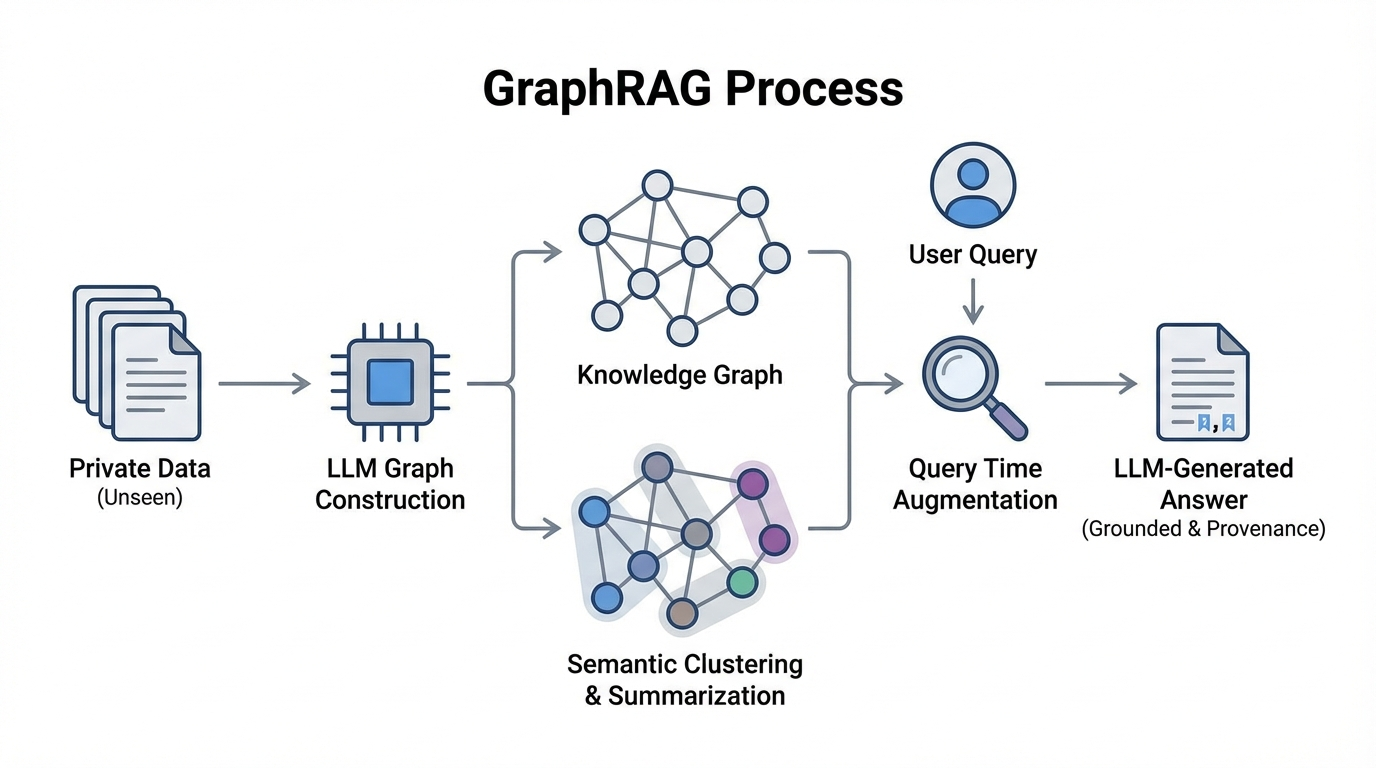
\includegraphics[width=\textwidth,height=0.7\textheight,keepaspectratio]{../images/graphrag.jpg}
        \caption{GraphRAG 分层索引架构}
      \end{figure}
    \end{column}
  \end{columns}
\end{frame}

\begin{frame}
  \frametitle{图增强检索：CGR³ \cite{xu2024cgr3}}

  \begin{columns}[T]
    \begin{column}{0.38\textwidth}
      \small
      \begin{block}{核心贡献}
        扩展三元组 KG，融入\textbf{时空、来源}等上下文信息
      \end{block}

      \vspace{0.2cm}

      \begin{block}{CGR³ 范式}
        \begin{enumerate}
          \item \textbf{Retrieve}：候选实体和上下文
          \item \textbf{Rank}：基于上下文排序
          \item \textbf{Reason}：判断信息是否充足
        \end{enumerate}
      \end{block}

      \vspace{0.2cm}

      \begin{block}{关键发现}
        上下文信息对 KG 补全和问答任务\textbf{至关重要}
      \end{block}
    \end{column}

    \begin{column}{0.58\textwidth}
      \begin{figure}
        \centering
        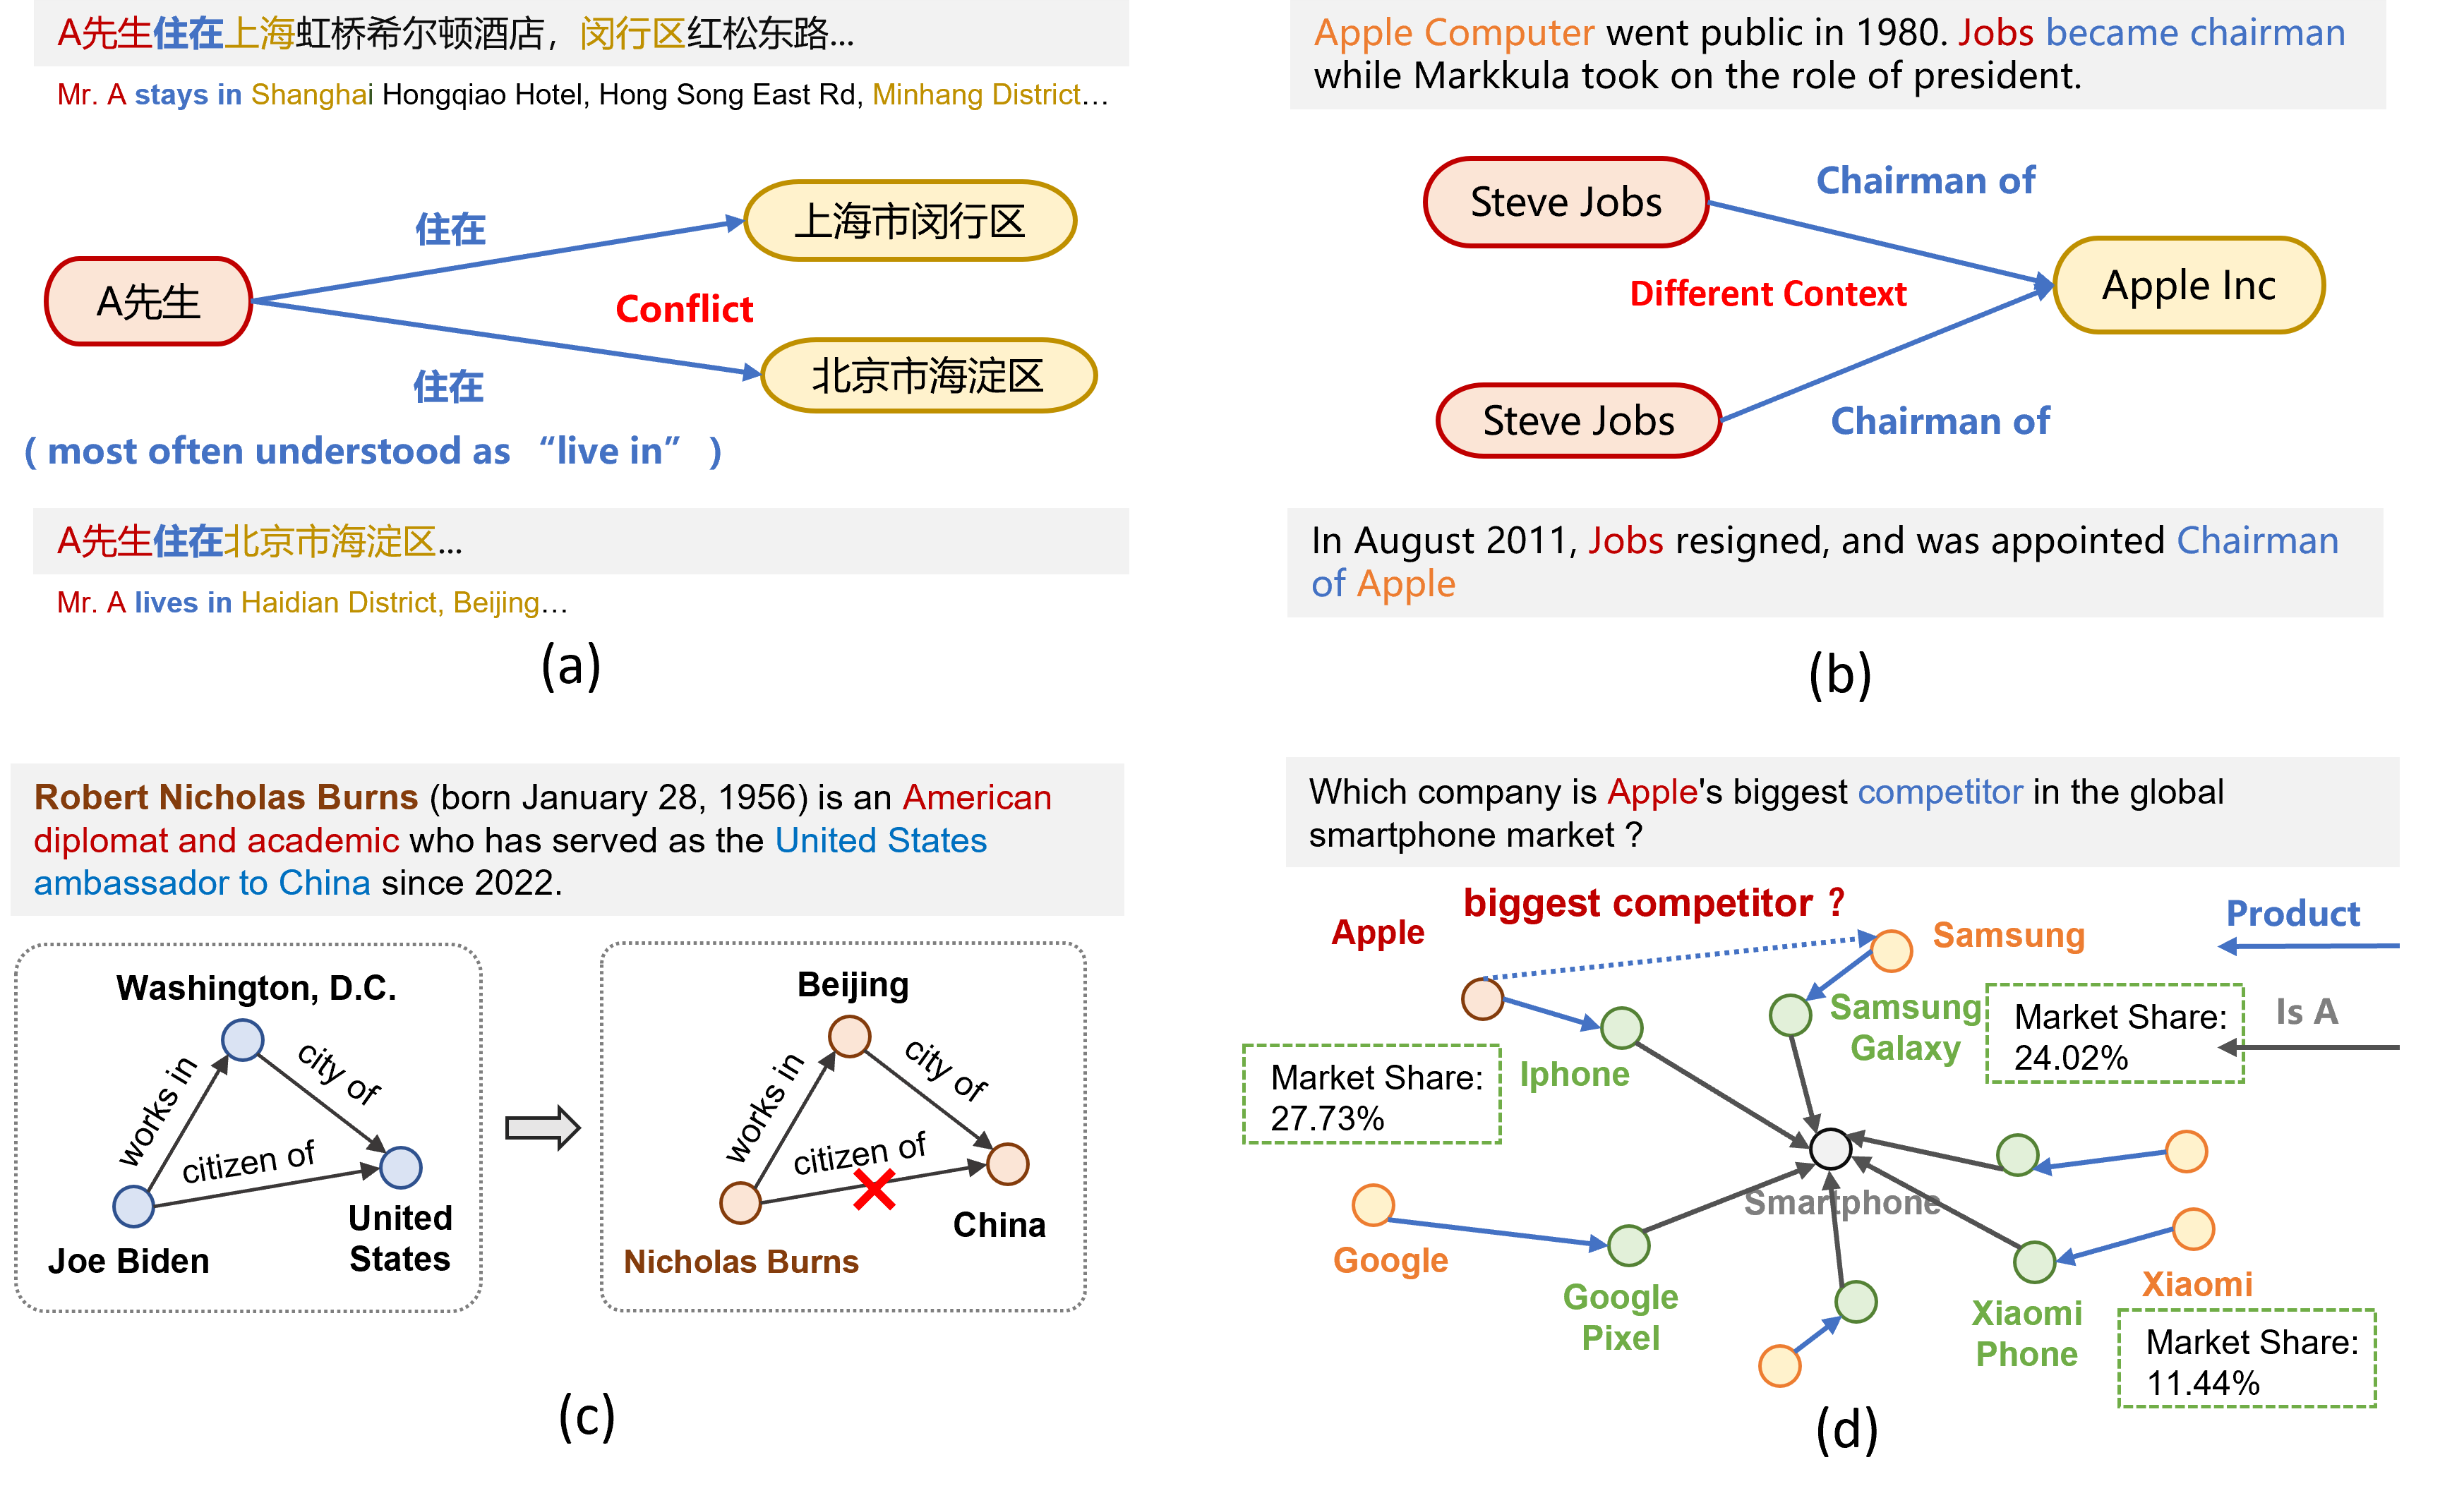
\includegraphics[width=\textwidth]{../images/cgr3.png}
        \caption{传统三元组 KG 的四个局限性}
      \end{figure}
      \tiny
      (a) 上下文丢失导致矛盾 (b) 无法区分相同关系的不同事实 \\
      (c) 规则推理忽略上下文 (d) 难以回答超出三元组范围的问题
    \end{column}
  \end{columns}
\end{frame}

\begin{frame}
  \frametitle{图增强检索：其他代表性工作}

  \begin{columns}[T]
    \begin{column}{0.32\textwidth}
      \begin{block}{RAPTOR \cite{sarthi2024raptor}}
        \small
        \textbf{递归抽象处理}
        \begin{itemize}
          \item 文本块聚类
          \item 生成层次化摘要树
          \item QuALITY 基准提升 20\%
        \end{itemize}
        \vspace{0.1cm}
        \tiny ICLR 2024, Stanford
      \end{block}
    \end{column}

    \begin{column}{0.32\textwidth}
      \begin{block}{Think-on-Graph \cite{sun2024tog}}
        \small
        \textbf{LLM$\otimes$KG 范式}
        \begin{itemize}
          \item LLM 作为代理探索 KG
          \item 束搜索交互式推理
          \item 9 个 KGQA 中 6 个 SOTA
        \end{itemize}
        \vspace{0.1cm}
        \tiny ICLR 2024, IDEA Research
      \end{block}
    \end{column}

    \begin{column}{0.32\textwidth}
      \begin{block}{HippoRAG \cite{gutierrez2024hipporag}}
        \small
        \textbf{海马体索引理论}
        \begin{itemize}
          \item LLM + KG + PPR
          \item 模仿人类长期记忆
          \item 多跳 QA \textbf{最高}提升 20\%
        \end{itemize}
        \vspace{0.1cm}
        \tiny NeurIPS 2024, Ohio State
      \end{block}
    \end{column}
  \end{columns}

  \vspace{0.4cm}

  \begin{alertblock}{共同趋势}
    图结构 + LLM 推理能力的结合，各有侧重：层次摘要、交互探索、联想记忆
  \end{alertblock}
\end{frame}

\begin{frame}
  \frametitle{Agent Memory：ExpeL \cite{zhao2024expel}}

  \begin{block}{核心问题}
    LLM Agent 如何在\textbf{不更新参数}的情况下从经验中学习？
  \end{block}

  \begin{columns}[T]
    \begin{column}{0.55\textwidth}
      \begin{block}{方法}
        \begin{enumerate}
          \item \textbf{经验收集}：Agent 与环境交互，存储成功/失败轨迹
          \item \textbf{洞察提取}：用 LLM 从轨迹中提取高层规则
          \item \textbf{推理调用}：检索相关洞察和过去经验辅助决策
        \end{enumerate}
      \end{block}

      \begin{block}{关键发现（AAAI 2024 Oral）}
        \begin{itemize}
          \item HotpotQA：洞察更重要（36\% vs 31\%）
          \item ALFWorld：轨迹回忆更重要（50\% vs 55\%）
          \item 不同任务需要不同的记忆形式
        \end{itemize}
      \end{block}
    \end{column}

    \begin{column}{0.42\textwidth}
      \begin{alertblock}{启示}
        \textbf{两种记忆形式}：
        \begin{itemize}
          \item 具体轨迹（episodic）
          \item 抽象洞察（semantic）
        \end{itemize}
        \vspace{0.2cm}
        Context Graph 需要同时支持这两种形式
      \end{alertblock}
    \end{column}
  \end{columns}
\end{frame}

\begin{frame}
  \frametitle{Agent Memory：A-Mem \cite{xu2025amem}}

  \begin{columns}[T]
    \begin{column}{0.55\textwidth}
      \begin{block}{核心问题}
        现有记忆系统结构固定，缺乏\textbf{动态自组织}能力
      \end{block}

      \begin{block}{Zettelkasten 方法}
        \small
        \begin{enumerate}
          \item 每个记忆单元生成结构化属性
          \item 分析历史记忆，建立语义关联
          \item 新记忆触发旧记忆\textbf{属性更新}
          \item 记忆网络持续演化
        \end{enumerate}
      \end{block}

      \begin{block}{实验结果（NeurIPS 2025）}
        \small
        复杂推理性能\textbf{翻倍}，Token 消耗降低，6 个模型均优于 SOTA
      \end{block}
    \end{column}

    \begin{column}{0.42\textwidth}
      \begin{figure}
        \centering
        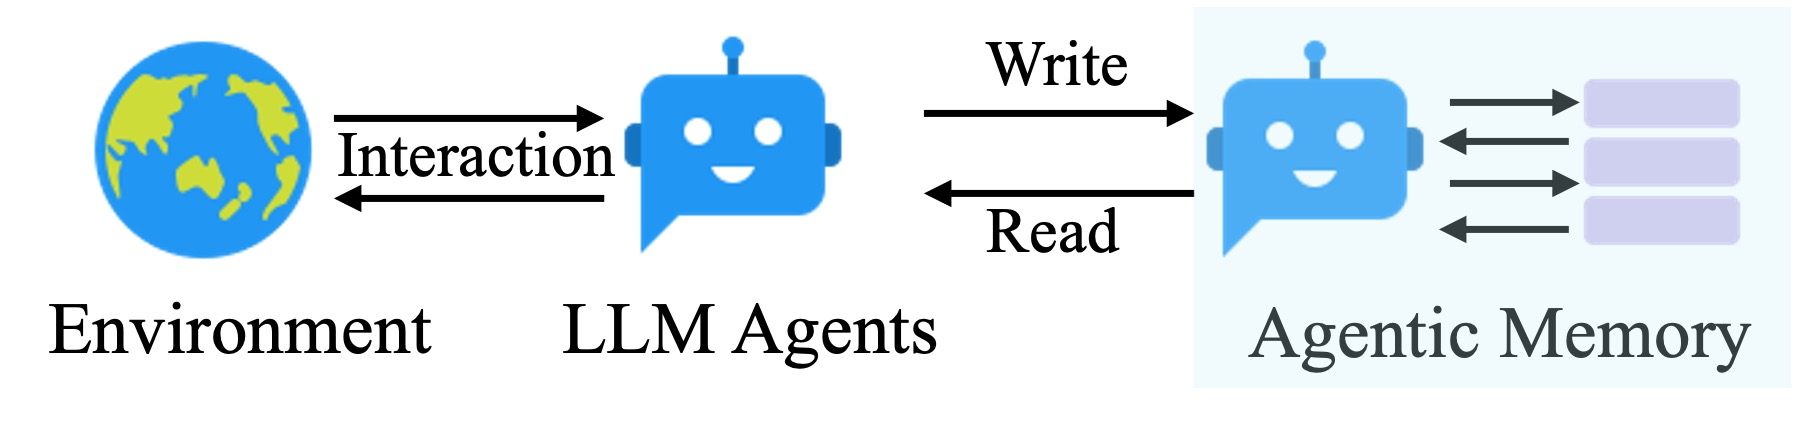
\includegraphics[width=\textwidth]{../images/a-mem.jpg}
      \end{figure}

      \begin{alertblock}{关键创新}
        \small
        \textbf{Agentic Memory}：记忆系统本身具有"代理性"，主动组织、链接、更新，而非被动存储-检索
      \end{alertblock}
    \end{column}
  \end{columns}
\end{frame}

\begin{frame}
  \frametitle{Agent Memory：可训练图记忆 \cite{xia2025trainable}}

  \begin{block}{核心问题}
    如何结合\textbf{隐式记忆}（可适应但不可解释）和\textbf{显式记忆}（可解释但难优化）？
  \end{block}

  \begin{columns}[T]
    \begin{column}{0.55\textwidth}
      \begin{block}{多层图记忆框架}
        \begin{enumerate}
          \item \textbf{底层}：状态机抽象 Agent 轨迹
          \item \textbf{高层}：元认知策略（人类可读）
          \item \textbf{优化}：基于 RL 的权重调整
        \end{enumerate}
      \end{block}

      \begin{block}{创新点}
        \begin{itemize}
          \item 从原始轨迹提取结构化决策路径
          \item 进一步蒸馏为高层策略
          \item 根据任务反馈动态调整策略权重
        \end{itemize}
      \end{block}
    \end{column}

    \begin{column}{0.42\textwidth}
      \begin{alertblock}{对 Context Graph 的启示}
        图结构需要：
        \begin{itemize}
          \item \textbf{多层次}：从具体到抽象
          \item \textbf{可训练}：根据反馈优化
          \item \textbf{可解释}：人类可理解
        \end{itemize}
      \end{alertblock}
    \end{column}
  \end{columns}
\end{frame}

\begin{frame}
  \frametitle{Agent Memory 方法对比}

  \small
  \begin{tabular}{p{2.2cm}|p{1.8cm}|p{3.5cm}|p{2cm}|p{1.2cm}|p{1.3cm}}
    \textbf{论文} & \textbf{核心问题} & \textbf{核心方法} & \textbf{记忆结构} & \textbf{可训练} & \textbf{发表} \\
    \hline
    ExpeL & 跨任务学习 & 提取 insights + 检索 & 列表 & \textcolor{red}{\ding{55}} & AAAI 24 \\
    \hline
    A-MEM & 记忆组织 & Zettelkasten 笔记网络 & 图（动态链接） & \textcolor{red}{\ding{55}} & NeurIPS 25 \\
    \hline
    Trainable Graph & 策略学习 & Meta-cognition + RL & 图（可训练权重） & \textcolor{darkgreen}{\ding{51}} & arXiv 25 \\
    \hline
    AgentDebug & 失败诊断 & 错误分类 + 根因定位 & N/A（诊断框架） & \textcolor{red}{\ding{55}} & arXiv 25 \\
    \hline
    AgentDiet & 效率优化 & 运行时轨迹压缩 & N/A（压缩方法） & \textcolor{red}{\ding{55}} & arXiv 25 \\
  \end{tabular}

  \vspace{0.3cm}

  \begin{alertblock}{研究空白}
    \begin{itemize}
      \item 现有工作主要在通用 QA 任务验证，\textbf{Coding 场景几乎未探索}
      \item 只有 Trainable Graph Memory 支持可训练，但未应用于代码任务
    \end{itemize}
  \end{alertblock}
\end{frame}

\begin{frame}
  \frametitle{现有方法的关键 Gap 与批判}

  \begin{columns}[T]
    \begin{column}{0.58\textwidth}
      \begin{block}{Gap 1：图结构设计缺乏共识}
        \footnotesize
        节点是什么？边表示什么？粒度如何选择？
      \end{block}

      \begin{block}{Gap 2：从"记录"到"学习"的鸿沟}
        \footnotesize
        大多数工作停留在"存储-检索"范式，无法主动学习
      \end{block}

      \begin{block}{Gap 3：领域特定应用的空白}
        \footnotesize
        现有工作主要在通用 QA 验证，\textbf{Coding 场景几乎空白}
      \end{block}
    \end{column}

    \begin{column}{0.38\textwidth}
      \begin{alertblock}{FlexRule 批判 \cite{flexrule2024critique}}
        \footnotesize
        单纯依赖历史轨迹 = 将\textbf{"先例误认为政策"}

        \vspace{0.1cm}

        轨迹是\textbf{"收据"}，不是\textbf{"食谱"}

        \vspace{0.1cm}

        \textbf{启示}：Context Graph 需区分\textbf{描述性} vs \textbf{规范性}知识
      \end{alertblock}
    \end{column}
  \end{columns}
\end{frame}

%==============================================================================
\section{研究方向探索}
%==============================================================================

\begin{frame}
  \frametitle{Coding Agent 任务全景}

  \small
  \begin{columns}[T]
    \begin{column}{0.48\textwidth}
      \begin{block}{1. 代码生成 (Code Generation)}
        \begin{itemize}
          \item 函数/类生成 (HumanEval, MBPP)
          \item 仓库级生成 (CodeAgentBench)
          \item 跨文件功能实现
        \end{itemize}
      \end{block}

      \begin{block}{2. Bug 修复 (Issue Resolution)}
        \begin{itemize}
          \item GitHub Issue 修复 (\textbf{SWE-bench})
          \item 自动程序修复 (APR)
          \item 回归修复
        \end{itemize}
      \end{block}

      \begin{block}{3. 漏洞检测与修复}
        \begin{itemize}
          \item 安全漏洞发现 (CodeMender, Spark)
          \item 漏洞根因分析
          \item 补丁生成
        \end{itemize}
      \end{block}
    \end{column}

    \begin{column}{0.48\textwidth}
      \begin{block}{4. 测试生成 (Test Generation)}
        \begin{itemize}
          \item 单元测试生成 (SWT-Bench)
          \item Fuzz 测试用例生成
          \item 测试覆盖率提升
        \end{itemize}
      \end{block}

      \begin{block}{5. 代码审查 (Code Review)}
        \begin{itemize}
          \item PR 审查 (Qodo, CodeRabbit)
          \item 代码质量检查
          \item 风格一致性检查
        \end{itemize}
      \end{block}

      \begin{block}{6. 代码理解与导航}
        \begin{itemize}
          \item 代码库问答
          \item 依赖分析
          \item 文档生成
        \end{itemize}
      \end{block}
    \end{column}
  \end{columns}
\end{frame}

\begin{frame}
  \frametitle{主任务选择：Bug 修复（SWE-bench）}

  \begin{columns}[T]
    % 第一列：为什么选择
    \begin{column}{0.32\textwidth}
      \begin{block}{为什么选择？}
        \footnotesize
        \begin{itemize}
          \item 最主流的 Coding Agent 任务
          \item 成熟的 benchmark 和 leaderboard
          \item 与漏洞检测相关
        \end{itemize}
      \end{block}

      \begin{alertblock}{CG 能回答}
        \footnotesize
        \begin{itemize}
          \item 为什么之前失败？
          \item 正确流程是什么？
          \item 哪条路径最可靠？
        \end{itemize}
      \end{alertblock}
    \end{column}

    % 第二列：要提升的指标
    \begin{column}{0.32\textwidth}
      \begin{block}{要提升的三个指标}
        \footnotesize
        \textbf{1. 成功率}
        \begin{itemize}
          \item 问题：重复失败
          \item CG：记录失败模式
        \end{itemize}

        \textbf{2. 效率}
        \begin{itemize}
          \item 问题：token 消耗大
          \item CG：轨迹压缩
        \end{itemize}

        \textbf{3. 持续学习}
        \begin{itemize}
          \item 问题：从零开始
          \item CG：跨任务迁移
        \end{itemize}
      \end{block}
    \end{column}

    % 第三列：具体例子
    \begin{column}{0.32\textwidth}
      \begin{block}{具体场景示例}
        \footnotesize
        \textbf{问}：为什么失败？\\
        \textcolor{gray}{答：项目用 gradle 不用 maven}

        \vspace{0.2cm}

        \textbf{问}：正确流程？\\
        \textcolor{gray}{答：图上路径清晰展示}

        \vspace{0.2cm}

        \textbf{问}：哪条路径可靠？\\
        \textcolor{gray}{答：A→B 成功率 95\%}
      \end{block}
    \end{column}
  \end{columns}
\end{frame}

\begin{frame}
  \frametitle{方向 1：Bug 修复中的失败学习}

  \begin{block}{问题设定}
    Coding Agent 在修复 Bug 时经常陷入循环：反复尝试相同失败方案
  \end{block}

  \begin{columns}[T]
    \begin{column}{0.55\textwidth}
      \begin{block}{Context Graph 的作用}
        \begin{enumerate}
          \item 存储每次修复尝试（成功和失败）
          \item 记录失败原因和错误类型
          \item 建立 Bug 模式 $\rightarrow$ 修复策略的映射
          \item 检索时优先排除已知失败路径
        \end{enumerate}
      \end{block}

      \begin{block}{相关工作}
        \cite{zhu2025fail} 提出 AgentErrorTaxonomy，\\
        但未结合图结构进行经验组织
      \end{block}
    \end{column}

    \begin{column}{0.42\textwidth}
      \begin{alertblock}{研究问题}
        \begin{itemize}
          \item 如何表示"失败原因"？
          \item 如何判断两个 Bug 是否相似？
          \item 如何从失败中提取可迁移的洞察？
        \end{itemize}
      \end{alertblock}
    \end{column}
  \end{columns}
\end{frame}

\begin{frame}
  \frametitle{备选方向：漏洞检测}

  \small
  \begin{tabular}{p{2.2cm}|p{4cm}|p{4cm}}
    \textbf{维度} & \textbf{Bug 修复} & \textbf{漏洞检测} \\
    \hline
    任务起点 & 已知 Issue 描述 & 未知，需主动发现 \\
    评估标准 & Resolved Rate & 检测率 + 误报率 \\
    知识依赖 & 项目代码逻辑 & 安全知识 (CWE/CVE) \\
    容错性 & 高（可多次尝试） & 低（误报代价高） \\
  \end{tabular}

  \vspace{0.3cm}

  \begin{columns}[T]
    \begin{column}{0.55\textwidth}
      \begin{block}{为什么 Bug 修复优先？}
        \begin{itemize}
          \item SWE-bench 基准成熟，便于验证效果
          \item 漏洞检测研究\textbf{几乎空白}，可作为后续
        \end{itemize}
      \end{block}
    \end{column}
    \begin{column}{0.42\textwidth}
      \begin{alertblock}{漏洞检测的机会}
        \begin{itemize}
          \item 安全知识图谱 + Agent
          \item CWE/CVE 模式学习
          \item 跨项目漏洞经验迁移
        \end{itemize}
      \end{alertblock}
    \end{column}
  \end{columns}
\end{frame}

%==============================================================================
\section{开放问题}
%==============================================================================

\begin{frame}
  \frametitle{Open Problems}

  \begin{columns}[t]
    % --- 第一栏：基础设计问题 ---
    \begin{column}{0.32\textwidth}
      \textbf{\textcolor{dotred}{\large $\bullet$} 图结构设计}
      \vspace{0.1cm}
      \hrule height 1pt
      \vspace{0.2cm}

      \footnotesize
      \textbf{Q1: 节点粒度}
      \begin{itemize}
        \item 每个 action 一个节点？
        \item 还是抽象成高层策略？
      \end{itemize}

      \vspace{0.15cm}

      \textbf{Q2: 边的语义}
      \begin{itemize}
        \item 时序？因果？语义相似？
        \item 如何混合多种关系？
      \end{itemize}

      \vspace{0.15cm}

      \textbf{Q3: 动态更新}
      \begin{itemize}
        \item 如何处理图的持续增长？
        \item 如何遗忘过时信息？
      \end{itemize}
    \end{column}

    % --- 第二栏：优化问题 ---
    \begin{column}{0.32\textwidth}
      \textbf{\textcolor{dotyellow}{\large $\bullet$} 学习与优化}
      \vspace{0.1cm}
      \hrule height 1pt
      \vspace{0.2cm}

      \footnotesize
      \textbf{Q4: 检索效率}
      \begin{itemize}
        \item 图太大时如何快速定位？
        \item 子图检索 vs 全图遍历？
      \end{itemize}

      \vspace{0.15cm}

      \textbf{Q5: 权重学习}
      \begin{itemize}
        \item 用 RL？监督学习？
        \item 如何定义奖励信号？
      \end{itemize}

      \vspace{0.15cm}

      \textbf{Q6: 探索 vs 利用}
      \begin{itemize}
        \item 过于依赖历史会错过新方案
        \item 如何平衡？
      \end{itemize}
    \end{column}

    % --- 第三栏：应用问题 ---
    \begin{column}{0.32\textwidth}
      \textbf{\large $\circ$ Coding 场景}
      \vspace{0.1cm}
      \hrule height 1pt
      \vspace{0.2cm}

      \footnotesize
      \textbf{Q7: Bug 表示}
      \begin{itemize}
        \item 如何编码 Bug 的语义特征？
        \item 如何判断 Bug 相似性？
      \end{itemize}

      \vspace{0.15cm}

      \textbf{Q8: 代码变化}
      \begin{itemize}
        \item 代码库更新后图如何同步？
        \item 历史经验是否仍有效？
      \end{itemize}

      \vspace{0.15cm}

      \textbf{Q9: 评估指标}
      \begin{itemize}
        \item 如何衡量 Context Graph 的价值？
        \item 超越 pass@k 的指标？
      \end{itemize}
    \end{column}
  \end{columns}
\end{frame}

%==============================================================================
\section{总结}
%==============================================================================

\begin{frame}
  \frametitle{文献分类}

  \begin{columns}[T]
    \begin{column}{0.48\textwidth}
      \begin{block}{图增强检索（GraphRAG 系列）}
        \small
        \begin{itemize}
          \item \textbf{GraphRAG} \cite{microsoft2024graphrag}：社区检测+分层摘要
          \item \textbf{RAPTOR} \cite{sarthi2024raptor}：递归抽象摘要树
          \item \textbf{Think-on-Graph} \cite{sun2024tog}：LLM$\otimes$KG 交互
          \item \textbf{HippoRAG} \cite{gutierrez2024hipporag}：海马体索引
          \item \textbf{CGR³} \cite{xu2024cgr3}：上下文增强 KG
          \item \textbf{GoR} \cite{zhang2025gor}：长文本处理
        \end{itemize}
      \end{block}

      \begin{block}{产业视角与评测}
        \small
        \begin{itemize}
          \item Foundation Capital \cite{foundationcapital2024context}：商业叙事
          \item Atlan \cite{atlan2024context}：架构指南
          \item FlexRule \cite{flexrule2024critique}：批判视角
          \item GraphRAG-Bench \cite{xiang2025graphragbench}：评测基准
        \end{itemize}
      \end{block}
    \end{column}

    \begin{column}{0.48\textwidth}
      \begin{block}{Agent Memory 系统}
        \small
        \begin{enumerate}
          \item \textbf{ExpeL} \cite{zhao2024expel} (AAAI 2024 Oral)
          \begin{itemize}
            \item 经验学习，洞察提取
          \end{itemize}

          \item \textbf{A-Mem} \cite{xu2025amem} (NeurIPS 2025)
          \begin{itemize}
            \item Zettelkasten 动态自组织
          \end{itemize}

          \item \textbf{可训练图记忆} \cite{xia2025trainable}
          \begin{itemize}
            \item 多层图 + RL 优化
          \end{itemize}

          \item \textbf{失败学习} \cite{zhu2025fail}
          \begin{itemize}
            \item 错误分类与调试框架
          \end{itemize}
        \end{enumerate}
      \end{block}
    \end{column}
  \end{columns}
\end{frame}

\begin{frame}
  \frametitle{总结与下一步}

  \begin{block}{核心观点}
    \begin{itemize}
      \item Context Graph = 图结构 + 决策痕迹 + 动态学习
      \item 学术（GraphRAG）和产业（决策追踪）是同一技术栈的不同视角
      \item Coding Agent 是一个有价值但尚未充分探索的应用领域
    \end{itemize}
  \end{block}

  \begin{block}{潜在研究方向}
    \begin{enumerate}
      \item \textbf{失败学习}：从 Bug 修复失败中构建可迁移的经验图
      \item \textbf{代码理解}：融合代码结构与探索轨迹的 Context Graph
    \end{enumerate}
  \end{block}

  \begin{alertblock}{需要进一步明确}
    \begin{itemize}
      \item 具体的研究问题和假设
      \item 实验设计和评估方法
      \item 与现有工作的差异化定位
    \end{itemize}
  \end{alertblock}
\end{frame}

% biblatex bibliography
\begin{frame}[allowframebreaks]
  \frametitle{参考文献}
  \printbibliography
\end{frame}

\end{document}
